% Penn -> Equifax (CRA reinvestigation, FCRA 1681i)
% Compile with XeLaTeX. Requires studentloan_core.tex and exhibit PDFs in the same folder.
\documentclass[12pt,letterpaper]{article}
\usepackage[left=1.25in,right=1.25in,top=1in,bottom=1in]{geometry}
\usepackage{fontspec}
\usepackage{graphicx}
\usepackage{parskip}
\usepackage{enumitem}
\usepackage{titlesec}
\usepackage{booktabs}
\usepackage{array}
\usepackage{pdfpages}
\titleformat{\subsection}{\normalfont\bfseries\scshape}{\thesubsection}{1em}{}
\begin{document}

\begin{center}
  \textbf{VIA CFPB PORTAL --- WRITTEN RECORD PRESERVED} \\
  \textbf{Date:} \underline{\today}
\end{center}

\begin{tabular}{@{}ll}
  \textbf{To:}   & Equifax Information Services LLC \\
                 & P.O. Box 740256, Atlanta, GA 30374 \\
                 & \\
  \textbf{From:} & Ash Le' A. Penn \\
                 & 17548 NW Springville Rd \#9, Portland, OR 97229 \\
\end{tabular}

\vspace{1em}\hrule\vspace{1em}

\textbf{Consumer:} Ash Le' A. Penn \quad \textbf{SSN:} XXX-XX-7755 \quad \textbf{DOB:} 02/15/1988 \\
\textbf{Report:} Equifax Confirmation No.\ 6060535900 (March 1, 2026) \\
\textbf{Re:} \textbf{Official FCRA Dispute and Reinvestigation Demand (15 U.S.C. \S~1681i)}

\vspace{1em}
\textbf{Attached Exhibits:} (1) Driver's License \& Utility Bill; (2) Equifax report 09/24/2024; (3) Equifax report 03/01/2026; (4) Midland Credit pre-legal notice 12/30/2024; (5) Comcast Notice of Dispute 04/03/2025; (6) copy of this dispute.

\vspace{1em}\hrule\vspace{1em}

To Whom It May Concern:

This is an official dispute and demand for reasonable reinvestigation under 15 U.S.C.\ \S~1681i regarding multiple inaccurate, re-aged, and obsolete tradelines. Equifax must also assure maximum possible accuracy under 15 U.S.C.\ \S~1681e(b).

\input{studentloan_core.tex}

\subsection*{Additional Tradelines Disputed}
\begin{itemize}[noitemsep]
  \item \textbf{Oregon Credit Systems *1645 (orig.\ GMC Properties Corp).} The reported balance is inflated from the \$15,632 original to \$20,508 and is unvalidated. Correct the balance and validate, or delete.
  \item \textbf{Steel Lending Group *3419.} The deficiency is barred under Oregon UCC Article 9 (ORS 79.0611/79.0614/79.0616, 79.0626) for failure of mandatory pre- and post-sale notice; reporting a \$13,635 balance is inaccurate (\S~1681e(b)). Correct or delete.
  \item \textbf{Exeter Finance *1001.} Exeter reports an active \$19,095 charge-off balance on a debt it sold to Midland Credit Management (which separately reports \$16,103 on the same debt). Double-reporting an active balance on a sold debt is inaccurate. Correct to \$0/sold or delete.
  \item \textbf{Eastern Account System *7892 (orig.\ Comcast).} The \$162 balance is actively disputed and is not marked ``disputed by consumer'' (FDCPA \S~1692e(8)). Mark disputed or delete.
\end{itemize}

\subsection*{Demands}
\begin{enumerate}[label=\arabic*., leftmargin=*]
  \item Reinvestigate the ten student-loan tradelines and require the furnisher to substantiate the Date of First Delinquency it reports; if it cannot be substantiated, delete the tradelines as inaccurate and obsolete under \S~1681c(a).
  \item Delete any Default Resolution Group collection tradeline that does not map to an originating loan (ten reported vs.\ nine loans).
  \item Correct or delete the four collection tradelines above.
  \item If any item is ``verified,'' provide the method of verification (\S~1681i(a)(7)).
  \item Respond in writing within 30 days.
\end{enumerate}

Failure to conduct a reasonable investigation and continued reporting of re-aged, inaccurate, and obsolete information is a willful and negligent violation of the FCRA.

\vspace{1.5em}\noindent Respectfully, \\ \vspace{1em}
\noindent 
\includegraphics[width=2.5in]{signature.jpg} \\
\textbf{Ash Le' A. Penn}

\newpage \includepdf[pages=-]{ID.png}
\newpage \includepdf[pages=-]{Proof_of_Address.pdf}
\newpage 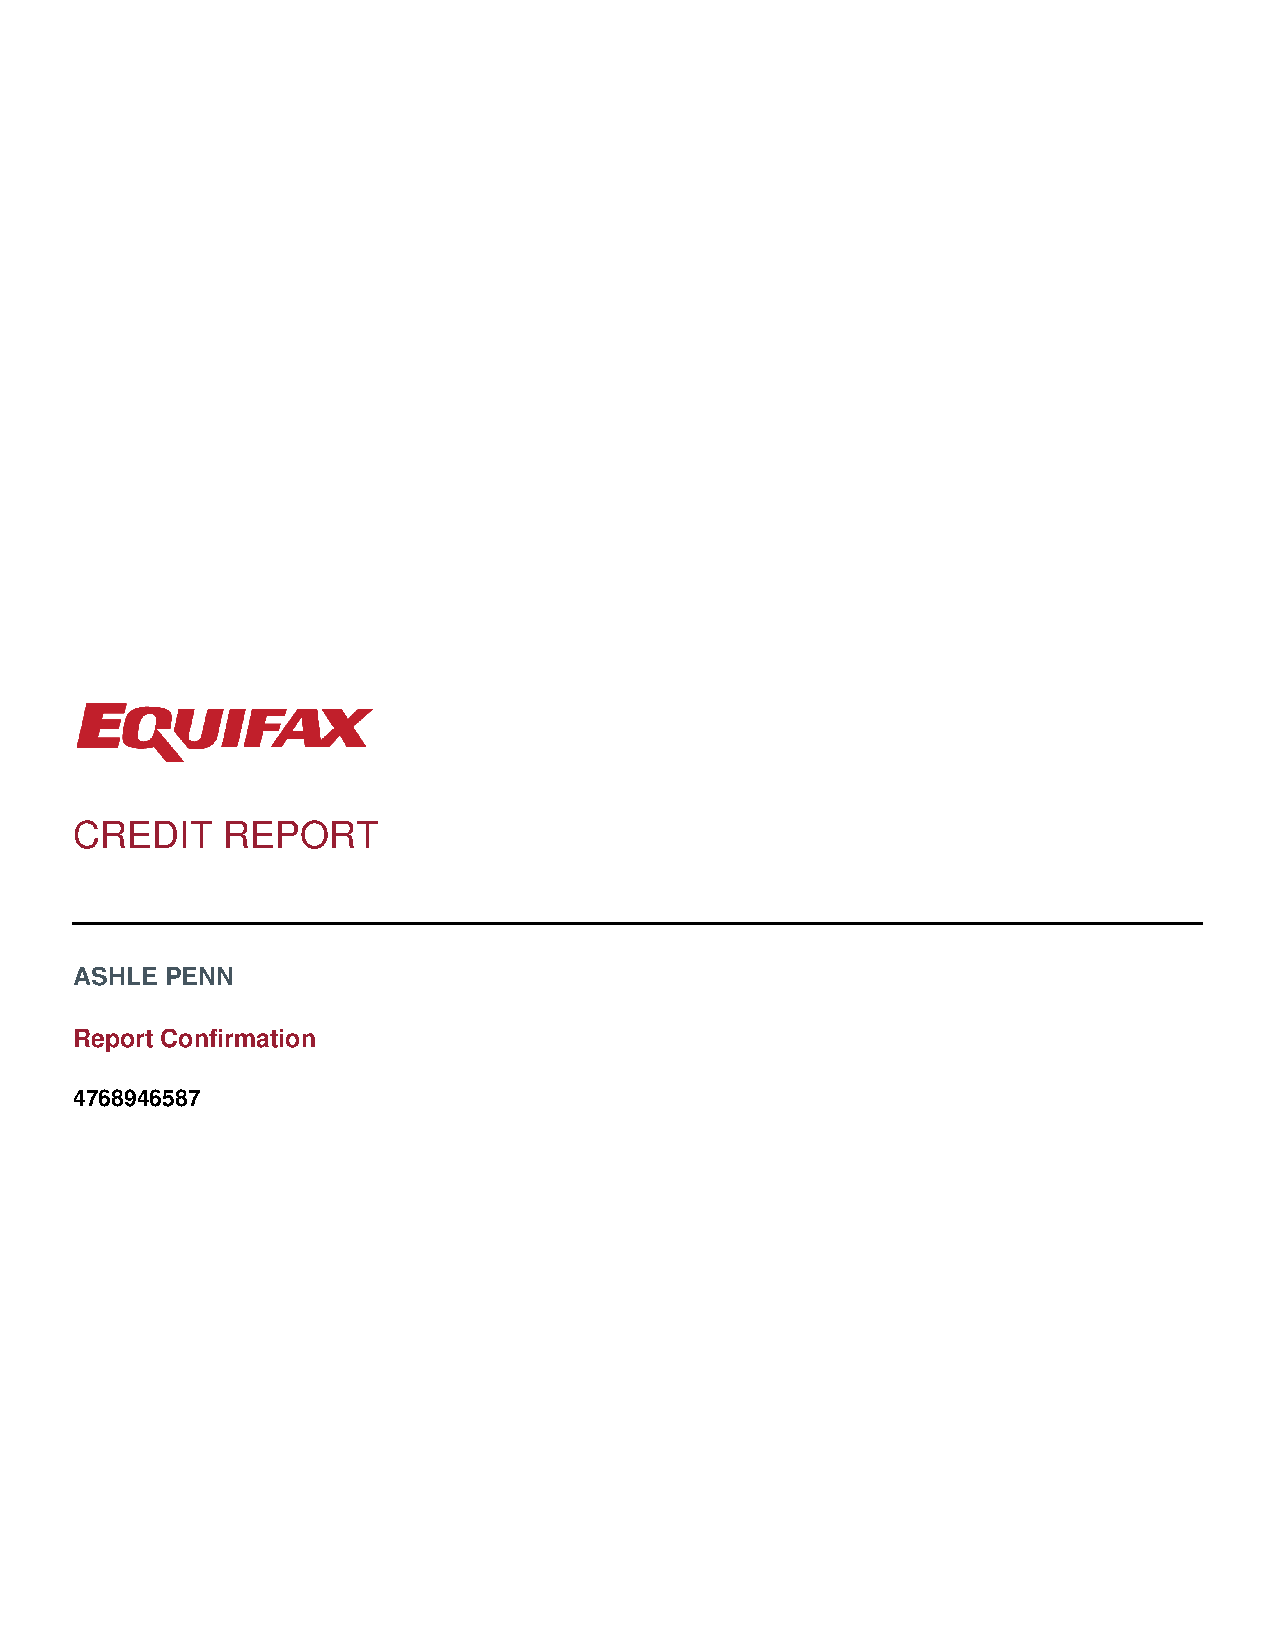
\includepdf[pages=-]{EQUIFAX_9.24.24.pdf}
\newpage \includepdf[pages=-]{EQUIFAX_3.1.26.pdf}
\newpage \includepdf[pages=-]{Gmail - Your Balance With EXETER FINANCE LLC (1).pdf}
\newpage \includepdf[pages=-]{Notice of Dispute (NOD).pdf}
\end{document}
